\documentclass[a4paper,12pt]{article}
\usepackage[utf8]{inputenc}
\usepackage[french]{babel}
\usepackage[T1]{fontenc}
\usepackage[top=2cm,bottom=2cm,left=2cm,right=2cm]{geometry}
\usepackage{graphicx}
\usepackage{wrapfig}
\usepackage{url}

\begin{document}

\begin{titlepage}
	\begin{center}
		\Large{Année universitaire 2016-2017}\\
		\Large{Université de Caen Basse-Normandie}\\[1cm]
		
		\huge{Rapport sur le premier semestre}\\
		\vspace{3cm}
		
		Alexis Carreau\\
		Thomas Lécluse\\
		Emma Mauger\\
		Théo Sarrazin\\
		
	\normalsize{\textit{ ~ L2 Informatique}}\\
		\medskip
		\vspace{2cm}
		
	\end{center}
\end{titlepage}

\tableofcontents
\newpage

\section{Introduction}

	\subsection{Présentation}
	Nous avons choisi de réaliser l'IDE (Environnement de Développement Intégré), car nous voulions créer un outil que nous pourrions utiliser par la suite. Ce sujet nous semblait donc intéressant à faire.
	
	Un IDE fournit des facilités au programmeur pour le développement logiciel. Il a pour but de maximiser la productivité du programmeur. Il contient généralement :
	\begin{itemize}
		\item un éditeur de texte, 
		\item un interpréteur, 
		\item un debugger,
		\item un compilateur,
		\item des options avancées comme la recherche de termes, l'auto-complétion, la coloration syntaxique...
	\end{itemize}
	
	Pour notre projet, nous nous inspirons de logiciels déjà existants, tels que Spider, Pycharm, Eclipse ou encore Emacs.
	\begin{figure}[h!]
		\begin{center}
			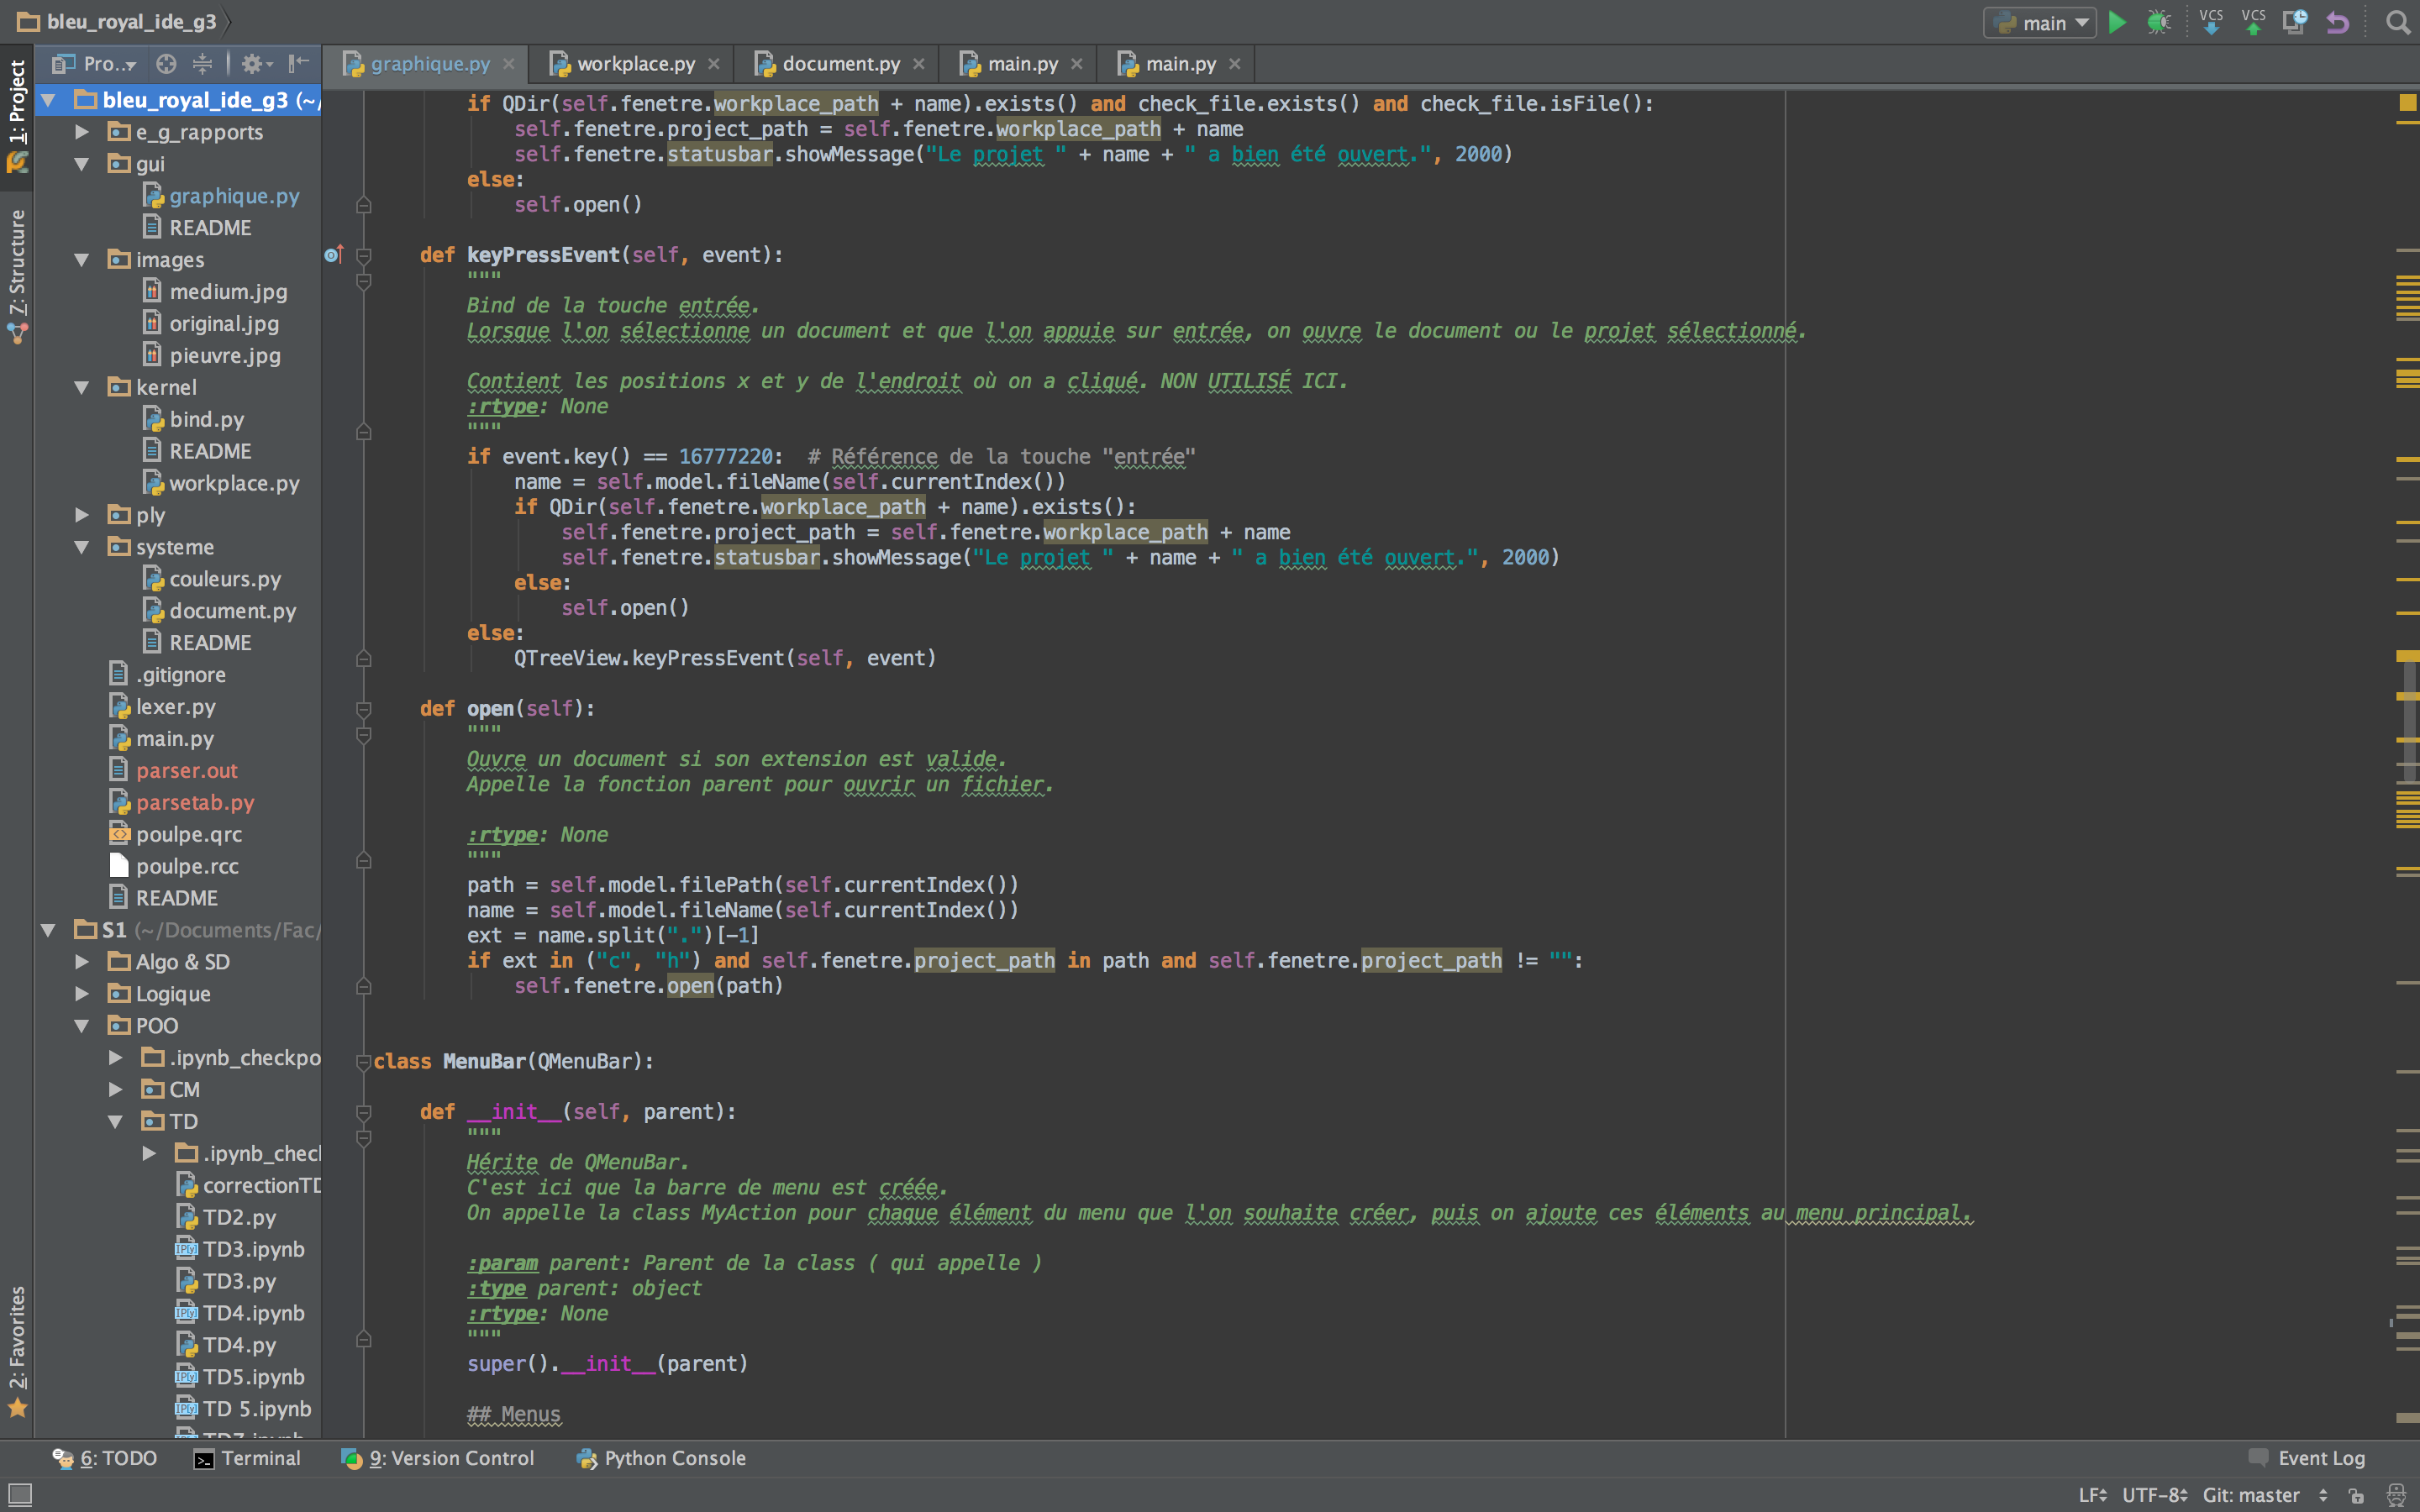
\includegraphics[scale=0.3]{images/pycharm}
			\caption{Exemple d'IDE, ici Pycharm}
		\end{center}
	\end{figure}
	
	\subsection{Objectifs}
	
	Nous devons d'ici à la fin de l'année réaliser un IDE qui contiendra les éléments cités ci-dessus. Pour la coloration lexicale et l'analyse syntaxique du code nous utiliserons les programmes Lex et Yacc.
	
	\subsection{Déroulement et planning}
	
	Nous avons réparti équitablement le travail et le temps de travail de chacun. Il faut préciser que deux membres du groupe (Thomas et Théo) connaissaient déjà la bibliothèque graphique utilisée dans l'IDE, et partaient donc avec un avantage non négligeable. \\
	Les deux autres membres du groupe ont donc été aidés afin de leur expliquer les bases et de pouvoir démarrer sans trop de problèmes.\\
	
	Nous avons réparti les différentes tâches à effectuer pour le projet entre les membres du groupe. Certaines sont plus longues ou plus complexes, c'est pourquoi certains membres du groupe ont une liste moins remplie que d'autres. Il ne faut donc pas se fier uniquement à cette liste.\\
	
	\begin{itemize}
		\item Alexis : Navigation et gestion des projets
		\item Emma : Recherche bibliographique, architecture projet, découpage en modules, barre de menu
		\item Théo : Coloration syntaxique, analyse lexicale, interface graphique, gestion (sauvegarde, ouverture) des fichiers
		\item Thomas : Documentation, interface graphique, thème, apparence texte et fenêtre, barre de statut
		\item Tout le groupe : Rapports et présentation 
	\end{itemize}
	
\section{Détails techniques}

	\subsection{Bibliothèques utilisées}
	
	
	Nous avons choisi la bibliothèque graphique QT (version 4.8.7, prévue à la base pour le C++) ce pourquoi nous avons aussi eu besoin de PySide (version 1.2.4), qui fait le lien vers le langage Python (version 3.4).\\
	
	La raison de ce choix est le fait que QT est un outil puissant de par ses nombreuses fonctionnalités. Sa documentation est de plus très fournie car les utilisateurs de QT sont plus nombreux que ceux de Tkinter.
	
	\subsection{Techniques et logiciels employées}
	
	Nous programmons en Python, car c'est un langage qui est multi-plateforme, qui est facile d'appréhension, et qui permet de faire beaucoup de choses. De plus, se documenter est facile car beaucoup de gens l'utilisent, il existe donc plusieurs sites où l'on peut trouver des réponses en cas de problème (StackOverflow, OpenClassroom...).
	
	Nous avons choisi un style de programmation orienté objet, puisque logique dans un projet de cette envergure. L'objet nous permet de mettre en application les notions vues en cours, autant l'année dernière que cette année, ainsi que de personnaliser en ré-implémentant des classes de QT pour les adapter à nos besoins.\\
	
	Lex est un programme qui permet de reconnaître des tokens qui sont des éléments d'une chaîne de caractères, à l'aide de règles lexicales que l'on lui passe en entrée.\\
	Dans notre cas, nous utilisons Lex pour reconnaître les éléments que l'on écrit, afin de colorer ces derniers en fonction de leur rôle (identifiant, entier, déclaration...). Nous utilisons la sortie générée en la passant à un autre programme : Yacc.\\
	
	Yacc permet de générer un arbre syntaxique abstrait qui nous permet de vérifier que la syntaxe de notre code est correcte. Aussi, cela permet de proposer une complétion automatique en fonction de ce que l'on écrit.\\
	Nous devons également lui passer des règles, qui sont d'ordre grammaticales.
	
	\begin{figure}[h!]
		\begin{center}
			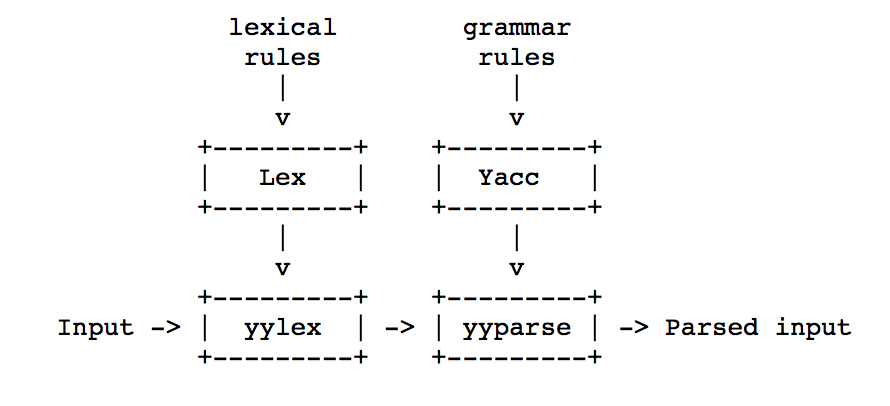
\includegraphics[scale=0.7]{images/schema_lex_yacc}
			\caption{Schéma résumant le fonctionnement de Lex et Yacc.}
		\end{center}
	\end{figure}
	
	\subsection{Bibliographie}
	
	Nous avons utilisé deux sites de documentation principalement sur QT et Pyside.
	\begin{itemize}
		\item \url{http://dinosaur.compilertools.net/}
		\item \url{http://epaperpress.com/lexandyacc/download/LexAndYaccTutorial.pdf}
		\item \url{http://www.drdobbs.com/web-development/prototyping-interpreters-using-python-le/184405580#l2}
		\item \url{http://tomassetti.me/autocompletion-editor-antlr/}
		\item \url{http://srinikom.github.io/pyside-docs/PySide/QtGui/}
		\item \url{doc.qt.io}
	\end{itemize}
	
\section{Structure générale}

	\subsection{Répartition en modules}
	
		Les différents modules sont répartis par thèmes. Nous avons :
		\begin{itemize}
			\item Un module pour l'interface graphique
			\item Un module pour la gestion des fichiers
			\item Un module pour la gestion des projets
			\item Un module pour la coloration syntaxique (avec Lex)
		\end{itemize}
		
	\subsection{Module graphique}
	
		On retrouve dans ce module tout ce qui est relatif à l'interface graphique (GUI).\\
		C'est là qu'est créée la fenêtre principale de l'application, où l'on va pouvoir créer, ouvrir, sauvegarder des fichiers et des projets.\\
		Nous n'hésitons pas à créer des classes afin de modifier les objets de QT pour les adapter en fonction de nos besoins. Cela permet aussi dans certains cas de compacter le code.
		On retrouve dans ce module ce qui est nécessaire pour :
	
			\subsubsection*{Créer une zone de texte}
			
			 	Nous utilisons pour cela l'objet "QTextEdit" de QT, qui est un widget permettant d'avoir une zone de texte. Nous nous en servons comme fenêtre d'éditeur, c'est donc ici que l'on pourra écrire du code.\\
			Le thème de l'application, (c'est-à-dire la couleur de fond et de la police ainsi que cette dernière) est relatif au QTextEdit. C'est également là que la couleur des éléments (tokens) sera modifiée par Lex en fonction de leur rôle.\\
			\begin{center}
				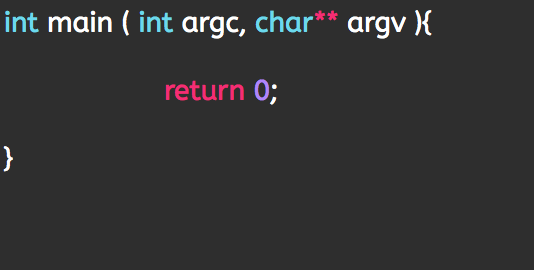
\includegraphics[scale=0.8]{images/QTextEdit}
				\vspace{0.5cm}
			\end{center}
			Nous avons ici une classe "Editeur" qui hérite de cet objet. Cela nous permet de paramétrer (couleurs, police et taille d'écriture) la zone de texte afin de pouvoir la créer plus facilement.\\
			
			\subsubsection*{Créer plusieurs onglets de code}
			
			 	C'est un QTabWidget que nous utilisons pour cela. Il va créer plusieurs "QTextEdit" (ou en supprimer si on ferme l'onglet), possède des fonctions et des raccourcis pour naviguer entre eux tous. \\
			Si aucun onglet n'est ouvert, le logo de notre groupe est affiché à la place.\\
			\begin{center}
				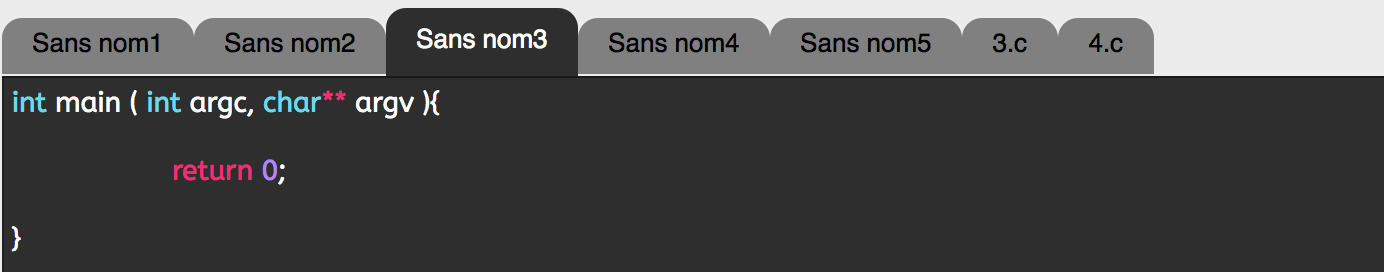
\includegraphics[scale=0.6]{images/QTabWidget}
				\vspace{0.5cm}
			\end{center}
			Nous avons créé une classe "TabWidget" qui hérite de cet objet. Un onglet est en fait un "QTextEdit", nous créons donc une nouvelle instance de notre classe "Editeur" pour chaque onglet. Le style des onglets, ainsi que le logo du groupe sont mis en place dans cette classe. On utilise pour cela des stylesheets de CSS.\\
			
			\subsubsection*{Créer une barre de menu}
			
				La barre de menu permet d'avoir toutes les fonctionnalités et éventuellement des raccourcis. On utilise une QMenuBar pour cela, qui va elle-même utiliser une "QAction" pour créer une action sur le menu. Une action contient un nom, éventuellement un raccourci et une fonction à exécuter. \\
			\begin{center}
				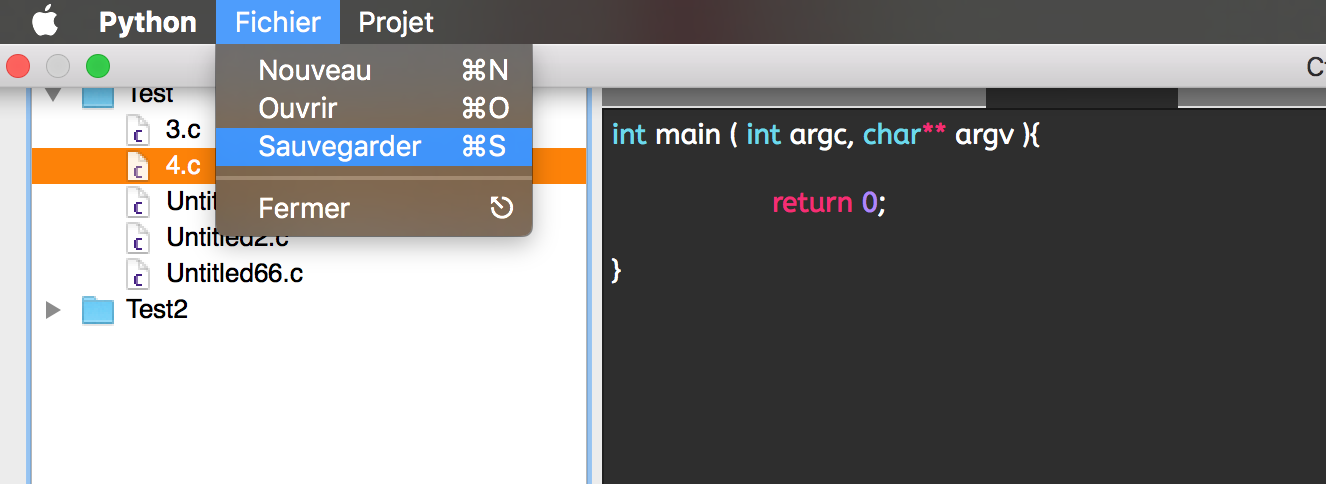
\includegraphics[scale=0.6]{images/QMenuBar}
				\vspace{0.5cm}
			\end{center}
			Nous avons ici deux classes. La première, "MyAction" hérite de "QAction" et permet tout simplement d'initialiser une action avec son nom, éventuellement un raccourci et une fonction à exécuter. Cela permet de compacter la création d'onglets dans notre menu.\\
			Ensuite nous avons une classe "MenuBar" qui hérite de "QMenuBar" et qui va créer toutes les instances de "MyAction" nécessaires à la créations des sous-menus et des onglets du menu. Les actions sont ensuite ajoutées aux menus.\\
			
			\subsubsection*{Mettre en place le navigateur de fichiers et de projets}
			
				Nous utilisons un "QTreeView" et un modèle "QFileSystemModel" qui nous permet d'afficher l'arborescence des fichiers et projets. C'est ce que l'on utilise pour ouvrir et naviguer dans les projets ouverts.\\
			\begin{center}
				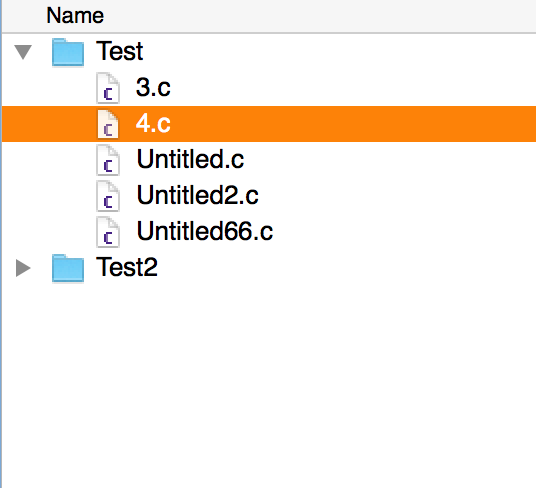
\includegraphics[scale=0.6]{images/QTreeView}
				\vspace{0.6cm}
			\end{center}
			Notre classe "TreeView" hérite de "QTreeView" et permet d'instancier correctement le navigateur pour, par exemple, lui demander de filtrer les fichiers pour n'afficher que les fichiers en .c et .h. On crée aussi des méthodes pour pouvoir ouvrir des projets et des fichiers en double-cliquant dessus mais elles sont placées dans un autre module.\\
			
			\subsubsection*{Modifier la taille du navigateur de fichier/de l'éditeur de code}
				Pour cela, nous utilisons un "QSplitter". Cela peut permettre, en fonction de la taille du projet et des répertoires imbriqués dans d'autres, de visualiser complètement les fichiers. Au contraire, on peut réduire le navigateur de fichier pour avoir une zone de code plus grande.\\
			\begin{center}
				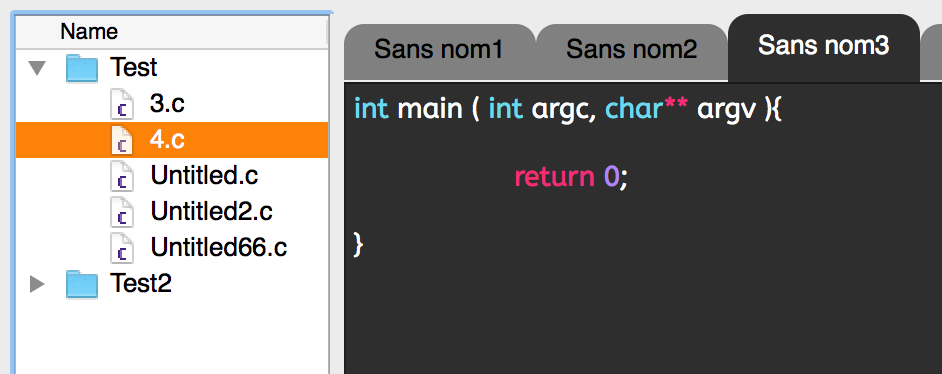
\includegraphics[scale=0.6]{images/QSplitter_1}
				\vspace{0.6cm}
			\end{center}

			\begin{center}
				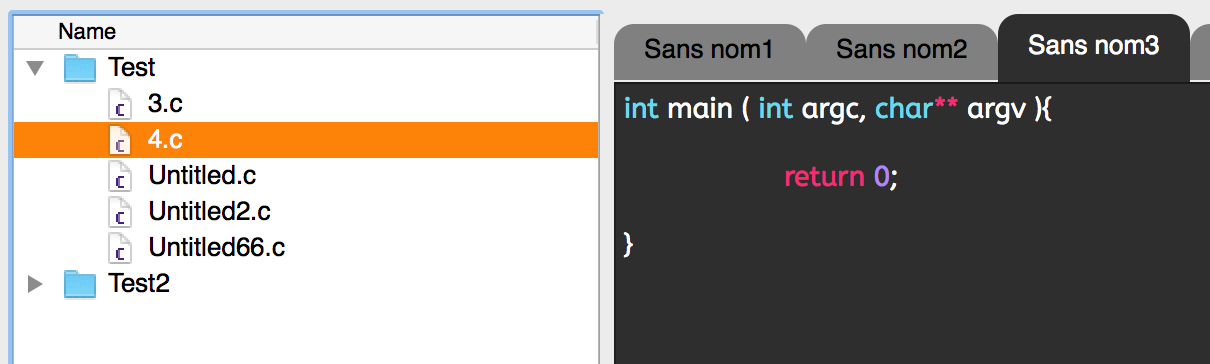
\includegraphics[scale=0.6]{images/QSplitter_2}
				\vspace{0.6cm}
			\end{center}
			Le QSplitter ne nécessite pas de modifications particulières. En fait on crée juste un objet "QSplitter", Et on ajoute les widgets de notre choix dedans. Ils seront donc dans une sorte de boîte dont on peut changer la taille.\\
			
			\subsubsection*{Afficher une barre de statut}
			
			 	Cela peut être pratique pour afficher des messages sans pour autant utiliser une popup. On y affiche généralement des informations (la plupart temporairement) comme la sauvegarde réussie d'un fichier, l'ouverture d'un projet, le nombre de lignes... L'objet QT qui permet cela est une "QStatusBar" et nous avons choisi de la placer tout en bas de l'application.\\
			\begin{center}
				
\includegraphics[scale=0.6]{images/QStatusBar}
				\vspace{0.6cm}
			\end{center}
			De même que pour le "QSplitter", pour l'usage que nous en avons, il n'est pas nécessaire de faire une classe qui hérite de QStatusBar. Il suffit juste de la créer et d'afficher des messages avec une méthode.\\
			
			\subsubsection*{Créer la fenêtre principale}
			
				Nous utilisons un "QWidget", qui est en fait une sorte de parent de tous les objets cités ci-dessus. Nous avons une classe "Fenetre" qui hérite de cet objet. C'est ici que l'on instancie tout les objets précédemment cités.\\
			\begin{center}
				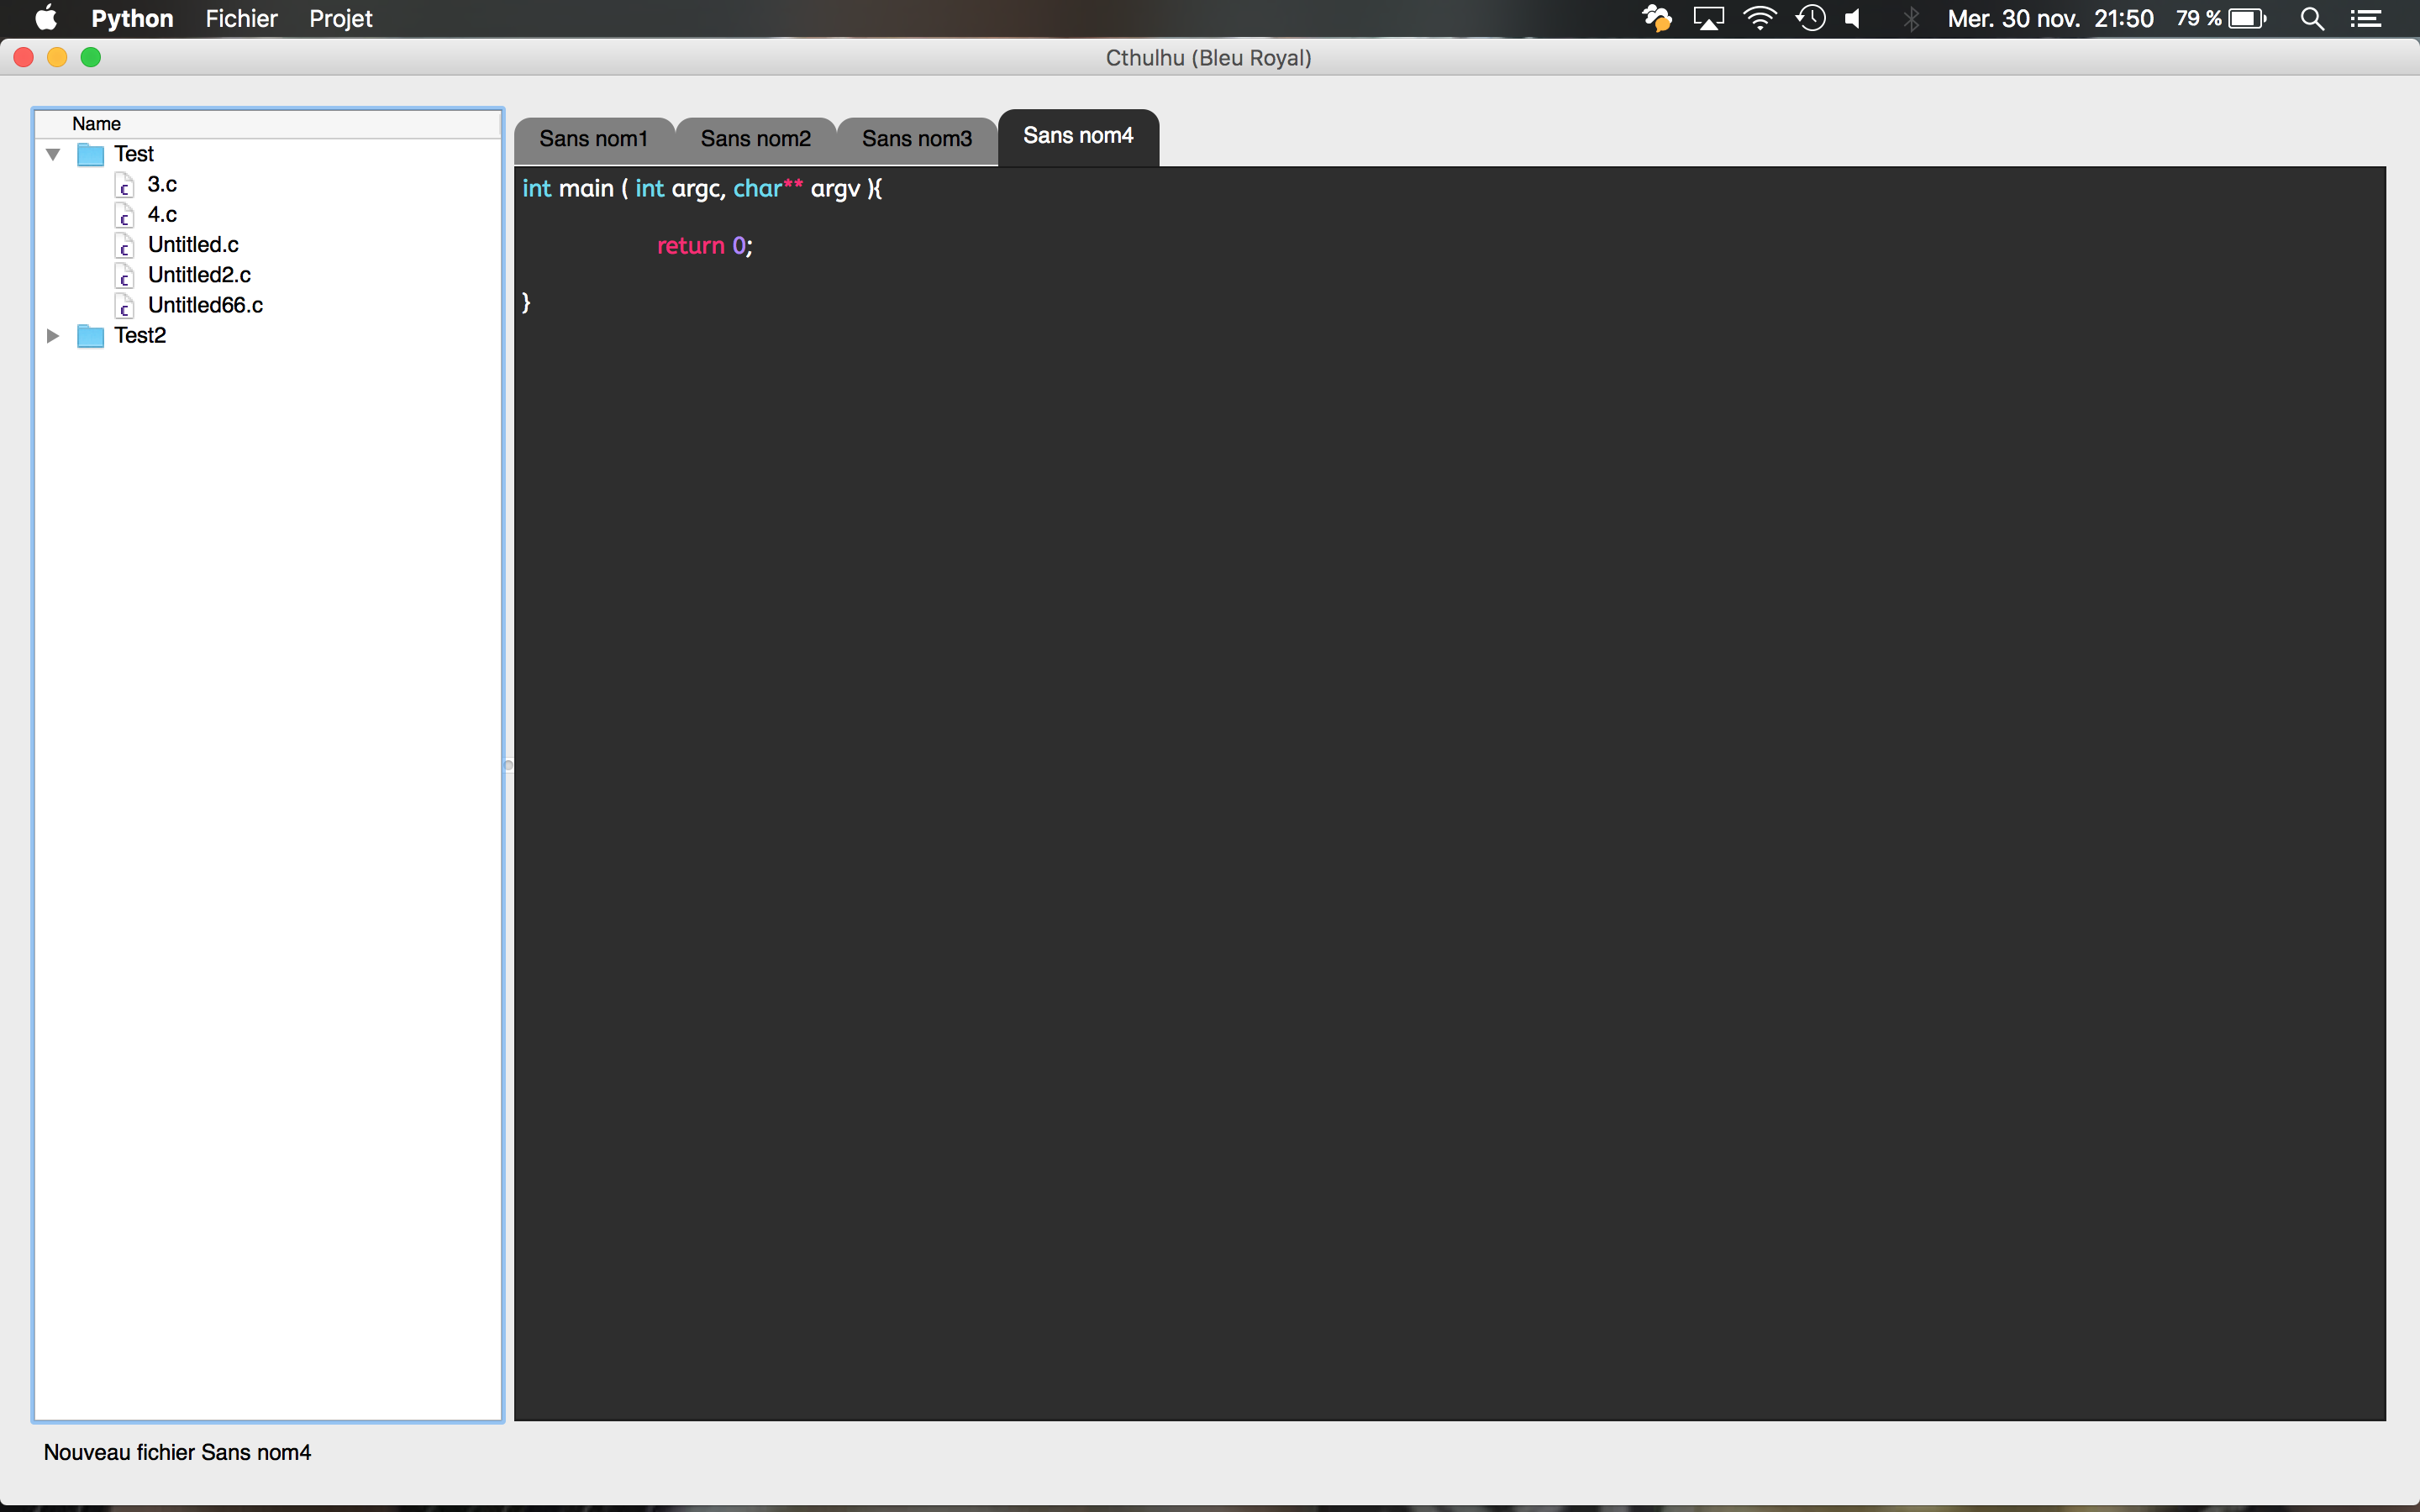
\includegraphics[scale=0.2]{images/QWidget}
				\vspace{0.6cm}
			\end{center}
			
		\subsubsection*{Schémas UML récapitulatifs}
		
			Les UMLs ci-dessous résument les héritages, les relations entre nos objets et ceux de QT ainsi que les relations entre nos modules. Nous les avons répartis en deux schémas pour des questions de lisibilité.
			
			\begin{figure}[h!]
				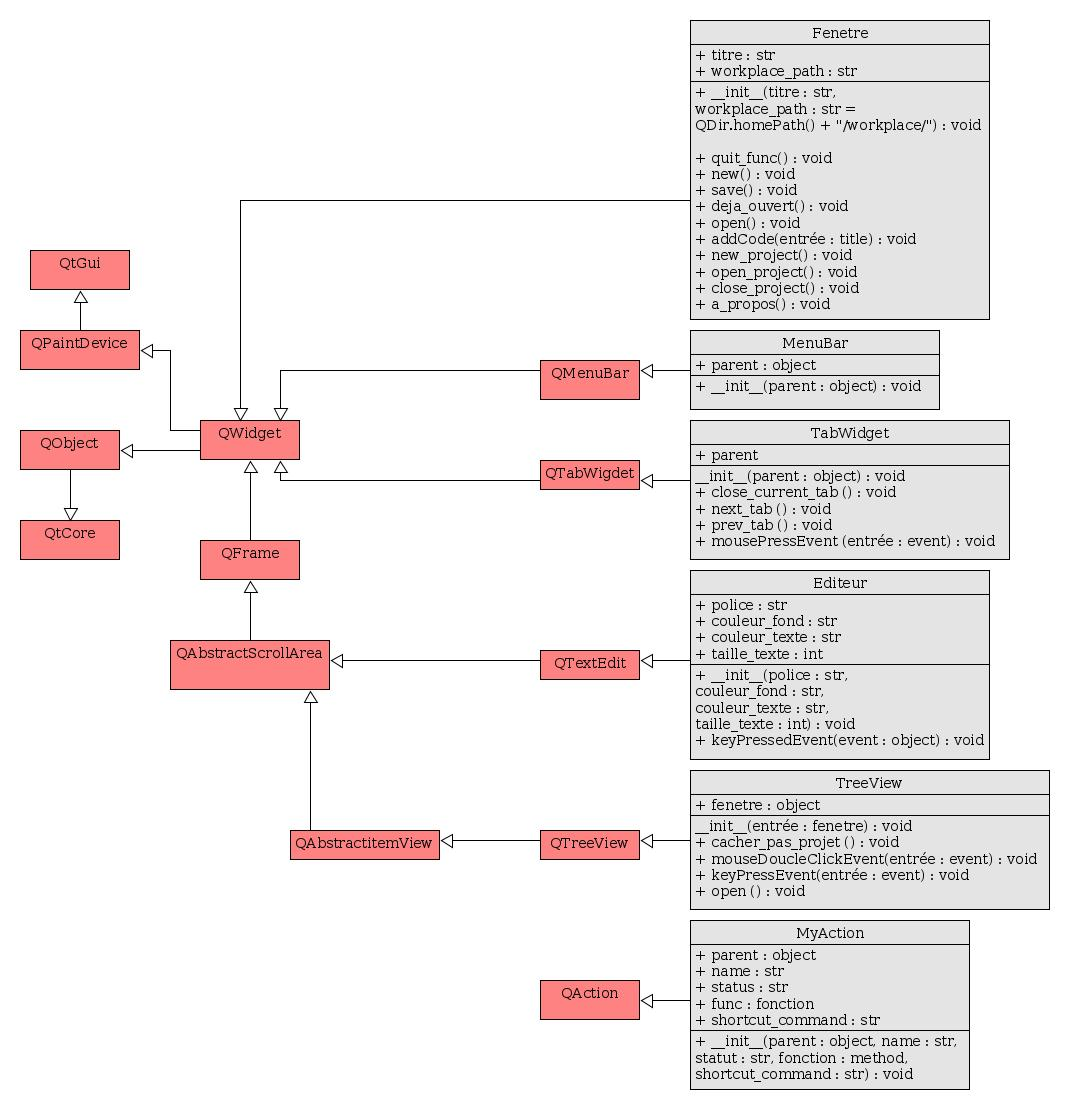
\includegraphics[scale=0.45]{images/uml_module_gui_heritage}
				\caption{Héritages avec les objets QT}
			\end{figure}
			
			\begin{figure}[h!]
				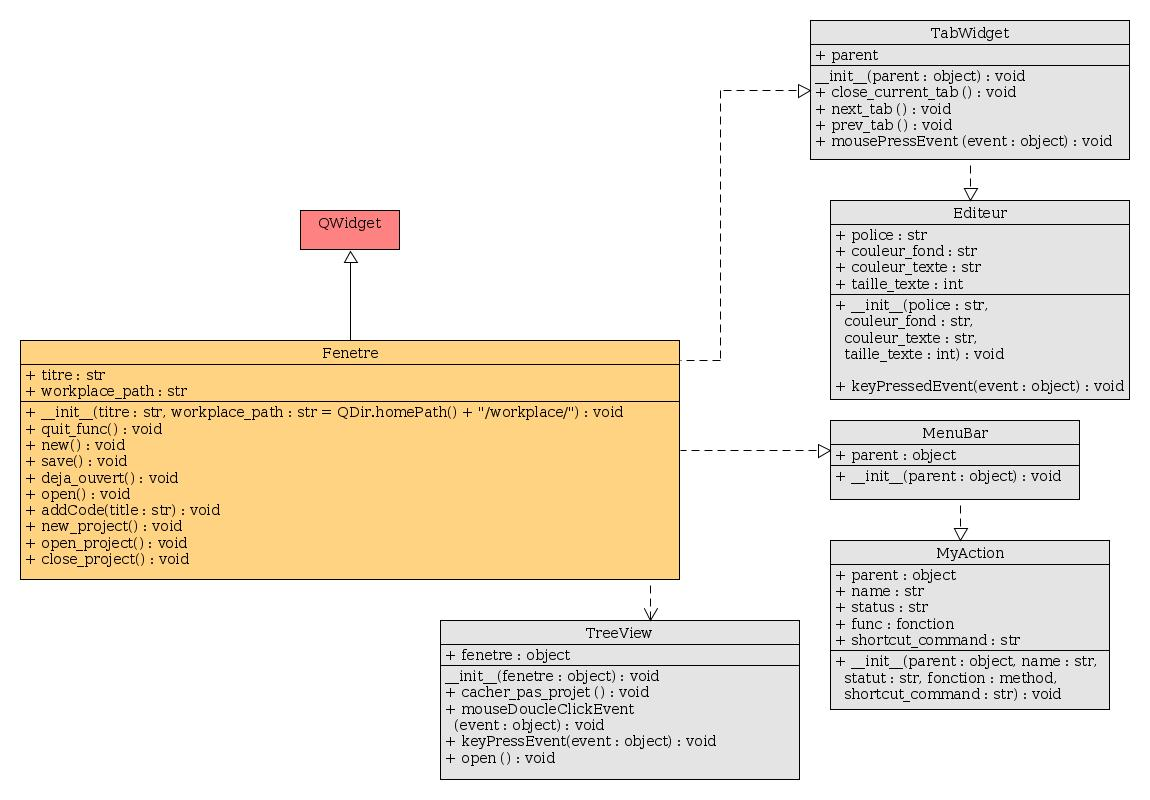
\includegraphics[scale=0.4]{images/uml_module_gui_relations}
				\caption{Relations entre nos objets}
			\end{figure}
			
		\newpage			
		\subsection{Modules de gestion des projets et des fichiers}
		
		Dans un IDE, la présence d’un navigateur de fichier s’impose afin d’avoir un certain confort pour parcourir l’arborescence de projets.\\
		Pour intégrer ce dernier dans notre IDE, nous avons utilisé la classe "QTreeview" comme vu ci-dessus dans le module graphique. Afin d'afficher les fenêtres d'ouverture, de création ou de sauvegarde, on utilise les styles de fenêtres du système, grâce à l'objet "QFileSystemModel". Par ailleurs, on filtre tous les documents afin de n'afficher que les fichiers en .c et en .h qui - pour l'instant - sont les seuls à nous intéresser.\\
		
		La gestion des projets se fait avec un système d'espace de travail, c’est-à-dire que les projets sont créés dans un répertoire "Workplace" à la racine de l’ordinateur. Un fichier de configuration en format ".xml" est ajouté automatiquement dans chaque projet créé, car cela permet de limiter - pour le moment - la création d’un projet en dehors de l’IDE et obliger la création dans répertoire "Workplace".\\
		
		Pour le moment, nous n'ouvrons que des fichiers qui appartiennent à des projets. On peut évidemment sauvegarder un fichier, et en créer un dans un projet. De plus, un même document ne peut être ouvert plusieurs fois.\\
		Lors de la modification, le fichier est chargé dans notre objet "Editeur" qui hérite du "QTextEdit" de QT.
		
		\begin{figure}[h!]
			\begin{center}
				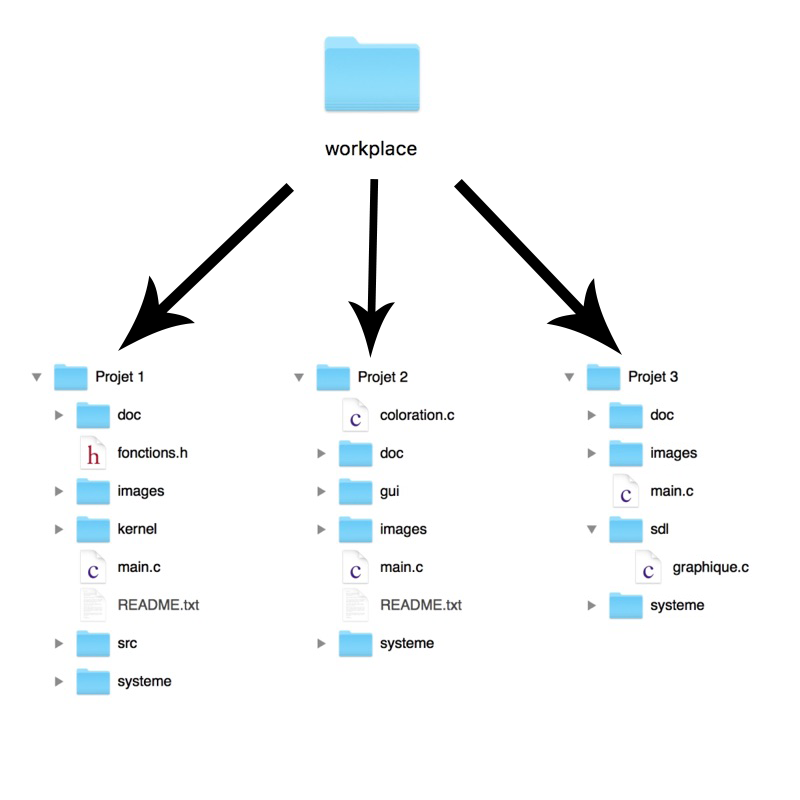
\includegraphics[scale=0.5]{images/nav_fic}
				\caption{Schéma gestion des projets et des fichiers}
			\end{center}
		\end{figure}
		
		\newpage
			
		\subsubsection*{Par la suite...}
		
				Nous comptons rendre possible la création de projets à partir de répertoires déjà existants. Cela permettra une plus grande souplesse pour l'utilisateur.\\
				De même pour l'ouverture et la création de fichiers, qui à terme, ne seront plus forcément liés aux projets. On devrait pouvoir ouvrir un fichier de n'importe où sans devoir l'ajouter dans un projet avant.\\
				
				Nous comptons également ajouter d'autres langages, comme le python ou le java (que nous utiliserons l'année prochaine) afin de proposer plus de contenu. Pour cela, il nous suffit de trouver les grammaires et les règles syntaxiques des langages concernés et de les ajouter. Ce ne sont donc pas des modifications majeures à effectuer.
			
		\subsection{Module coloration syntaxique}	
		
		Dans ce module on retrouve tout le code relatif à la coloration syntaxique. C’est ici que nous utilisons LEX pour l’analyse lexicale.  
		
		\subsubsection*{Coloration du code en temps réel :}

	Pour la coloration syntaxique nous utilisons l’objet "QSyntaxHighlighter" de QT. Cette objet prend un "QTextDocument" en paramètre, c’est ce "QTextDocument" qui verra son code coloré. Pour cela, on crée une classe qui hérite de "QSyntaxHighlighter" (que nous avons nommé "CodeHighLighter"), puis on ré-implémente la méthode "highlightBlock".\\
	 Cette méthode est appelée à chaque changement du texte dans le "QTextDocument", avec en paramètre le texte correspondant à la ligne en cours d’édition. C’est donc dans cette méthode que nous faisons appel à LEX afin de connaître les tokens trouvés par ce dernier puis grâce à la méthode "setFormat" de l’objet "QSyntaxHighlighter" nous colorons le texte.
	 
	 \begin{figure}[h!]
			\begin{center}
				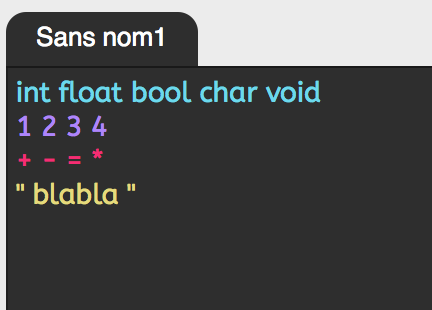
\includegraphics[scale=1]{images/color}
				\caption{Coloration de tokens}
			\end{center}
		\end{figure}
		
		Ces modifications de couleurs sont affichées via le "QTextEdit" (de notre classe "Editeur") qui contient le "QTextDocument". Les éléments trouvés par LEX sont classés en fonction de leur rôle, et c'est ce qu'on utilise pour les colorer.

		\subsubsection*{Fonctionnement de LEX}
		
	LEX fonctionne grâce à un principe de token. Un token est un mot-clé désignant le « type » du mot trouvé dans le code, comme par exemple un identifiant, un mot réservé par le langage, ou encore une chaîne de caractère. LEX nous retourne donc une liste contenant tous les tokens qu’il a trouvé, mais aussi la position à laquelle ils se trouvent dans le texte (caractère) mais aussi le numéro de la ligne.\\
	 Par la suite, grâce à la méthode "highlightBlock" de notre objet "CodeHighLighter", on utilise une fonction qui parcourt tous les tokens de LEX, cette fonction nous retourne pour chaque token sa position et la couleur associée à ce token, afin que l’on puisse colorer le code.
	
\section{Conclusion}

	\subsection{Programme pour le second semestre}
	Nous devons intégrer un compilateur pour le code c, et implémenter l'auto-complétion ainsi que l'analyse syntaxique. \\
	Nous avons quelques pistes : 
	\begin{itemize}
		\item pour le compilateur, il existe des compilateurs intégrés aux systèmes d'exploitation (sauf peut-être sous Windows), que l'on pourrait utiliser dans le cadre de notre projet,
		\item concernant l'analyse syntaxique, c'est le logiciel Yacc que l'on exploitera, grâce à ce qu'il génère, un arbre abstrait d'analyse. Pour le moment, nous arrivons à afficher (sur la console) ce que trouve (cf. partie sur Yacc) Yacc à chaque ligne de code,
		\item et enfin, pour l'auto-complétion, nous pensons récupérer l'arbre abstrait généré par Yacc pour proposer des éléments qui pourraient constituer une suite logique au code en train d'être écrit.
	\end{itemize}
	
	\subsection{Améliorations}
	Nous avons plusieurs idées d'améliorations pour notre IDE, sans compter le fait qu'il nous reste à intégrer Yacc et un compilateur. 
	
	\subsubsection*{La sauvegarde}
	
		Prévoir le cas où l'on souhaite fermer le logiciel sans avoir sauvé ses programmes avant. Il faut alors proposer à l'utilisateur de sauvegarder ses fichiers, et s'il le souhaite, quitter sans sauvegarder.
		
		\begin{figure}[h!]
			\begin{center}
				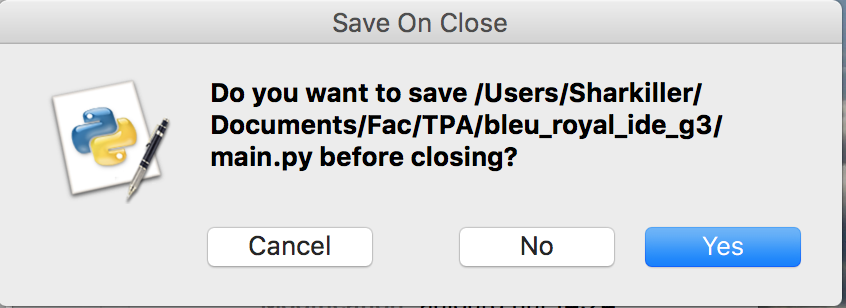
\includegraphics[scale=0.5]{images/save_on_close}
				\caption{Exemple de message de ce type sur IDLE}
			\end{center}
		\end{figure}
	
	\subsubsection*{La numérotation des lignes}
	
		Nous pensons aussi à numéroter les lignes de l'éditeur de texte, notamment dans le cas où on trouve des erreurs, pour pouvoir les récupérer et éventuellement indiquer à l'utilisateur la ligne qui comporte un problème. Ceci nous permettra d'afficher le nombre total de lignes, peut-être dans la barre de statut.
		
	\subsubsection*{Ajout de boutons}
		
		Notre interface IDE est globalement composée d'une zone de texte, d'un navigateur de fichiers et d'un menu. Le menu étant dans la barre de la fenêtre, le navigateur de fichier et la zone de texte prennent énormément de place, ce qui rend la fenêtre assez vide, ce pourquoi nous allons insérer des boutons pour que les paramètres importants soient accessibles facilement, tout en gardant une interface graphique épurée.
		
	\subsubsection*{Les projets et les fichiers}
	
		En ce qui concerne la gestion de projets et de fichiers, nous pensons faire en sorte de pouvoir gérer la suppression des projets des des fichiers directement depuis l'IDE, plutôt que de devoir le fermer, ouvrir son navigateur de fichiers puis les supprimer à la main (ou le faire en mode console depuis un terminal).
		
	\subsubsection*{Le debbuger}
	
		Le debugger nous semble être un outil utile lors de l'exécution de programmes, pour pouvoir permettre à l'utilisateur de repérer les bugs d'un programme, d'exécuter son programme pas-à-pas... Ce qui peut être un outil non négligeable pour les programmeurs.
		
	\subsubsection*{Le compilateur}
	
		Étant donné que notre IDE est prévu, à la base, pour du langage C (un langage compilé), il semble évident d'avoir un compilateur. Celui-ci ne sera disponible que lorsque le code écrit sera impeccable, dans le sens où il devra avoir passé l'analyse de Lex et les identifications de Yacc.
		
	\subsubsection*{Yacc}
	
		Yacc génère un arbre syntaxique abstrait de chaque terme trouvé dans le code qu'on lui passe. Ceci étant, il nous permettra de vérifier, grâce à des grammaires qui Lex génèrera, que le code est bien écrit et respecte bien la grammaire du langage dans lequel on code.
		
	\subsubsection*{Indentation automatique}
	
		Il nous faut aussi gérer l'indentation du code, quel qu'il soit, pour que l'utilisateur ne perde pas son temps à agencer son code.

\end{document}